\documentclass[letterpaper, 11 pt, conference]{article}
\usepackage{setspace}
\usepackage{listings}
\usepackage{color}
\usepackage{float}
\usepackage{graphicx}

\usepackage[utf8]{inputenc}
\usepackage[english]{babel}


\usepackage[english]{babel}


\usepackage[letterpaper,top=2cm,bottom=2cm,left=3cm,right=3cm,marginparwidth=1.75cm]{geometry}


\usepackage{amsmath}
\usepackage{graphicx}
\usepackage[colorlinks=true, allcolors=blue]{hyperref}
\title{Impact of Communal Attributes on Violent Crime in American Cities}
\author{Vedant Apte, Annmarie Adams, Hengze Ye, Matthew Boentoro, \\Dongyu Chen, Tien Ly, Loren Aguilar,  Yifan Shen, Anqi Liu}

\begin{document}
\maketitle

\begin{abstract}
Using a unique data set containing 1994 instances and providing 122 predictive communal attributes obtained from socio-economic data from the 1990 US Census, law enforcement data from the 1990 US LEMAS survey, and crime data from the 1995 FBI UCR, we developed and evaluated multiple machine learning models to predict the impact of communal attributes on the violent crime rate per 100K people. Several models suggest that omitted variables related to multiple attributes do not bias the predictions.
\end{abstract}

\section{Introduction}

Over the last several decades in American society, a period that has witnessed many great advances in all facets of life, the existence of violent crime has consistently plagued the nation. However, a continuous effort over the last 25 years to reduce violent crime in the United States has seen the violent crime rate decrease sharply. That being said, crime rates vary significantly between the states, with states with such as Alaska, New Mexico, and Tennessee experiencing much higher crime rates than states such as Maine, New Hampshire, and Vermont in modern American society.
\\
\\This variance in crime rates across different communities has engendered the debate of whether or not attributes specific to a community cause or prevent more crime. One side of this debate argues that various issues related to community backgrounds leads to a volatility in the absolute number of criminals, or the number of current criminals becoming active. For example, some conditions such as low income and the number of single parent homes play a role in encouraging criminals who are inclined to commit crimes to do so, and furthermore, commit them in a violent manner. The other side of the debate argues that communities and their unique properties have little to do with crime, because individuals, not their surrounding environments, are responsible for the decisions (good and bad) that they make.
\\
\\The empirical research on this topic presents mixed results. This contradiction is likely due to a lack of credible and accessible data on community backgrounds in the United States. Many researchers use different sources and proxies when making connections between community attributes and crime. For instance, when talking about the gun ownership rate in communities (which may affect the violent crime rate), the General Social Survey, the suicide rates by firearm (Moody and Marvell), and the circulation of gun magazines (Duggan 2001) all have been used as attempted proxies. It is difficult to say how well these truly estimate the gun ownership rate.
\\
\\To make definitive statements about the impact that community attributes have on the violent crime rate in a society, further research must be done. The conclusions drawn from this research are important not only for the general public's understanding, but also for policymakers at the local, state, and federal levels. By taking a prospective approach to the problem and predicting future crime rates given differing levels of specific communal attributes, the aforementioned governments can produce educated legislation and take actions that prevent the crime rate from rising in the first place, resulting in a safer America. Our project intends to analyze the \href{https://archive.ics.uci.edu/ml/datasets/Communities+and+Crime} {Communities and Crime Data Set} data set, found at the UC Irvine Machine Learning Repository, to draw these very conclusions by identifying numerical relationships between specific communal attributes and violent crimes per 100K. We will use this data set to train a machine learning model that can predict a normalized value for the violent crime per 100K given normalized inputs from one (or all) of three different communal attribute categories: family, race, and wealth. To obtain data to draw our conclusions, we will construct both a linear regression model as well as a neural network model, as all of our inputs and our output are continuous, numeric attributes. The following sections of this paper will elaborate on our choice of input attributes, analyze our approach when developing and choosing between the two aforementioned predictive machine learning models, present our results and data (graphical and numerical), and identify potential errors along with future courses of action.

\section{Literature Review}
Lots of research has been done to investigate factors which influence the crime rate. Additionally, more and more researchers are starting to apply machine learning methods to help them better analyze relationships between crime rate and various factors quantitatively. In this review, we focus on the influences of geological ranges, community backgrounds, and economic factors on the crime rate specifically, and present several pieces of machine learning based research. 
\\
\\First, some research in the field of crime variability among geological range studies has examined corrections. For regional comparisons in \cite{greenwade93}, the FBI divides the United States into four regions: Northeast, Midwest, South, and West. For 2019, the region with the lowest violent crime rate was the Northeast, with a rate of 292.4 per 100,000 residents, while the region with the highest violent crime rate was the West, with a rate of 413.5 per 100,000. For 2019, the region with the lowest property crime rate was the Northeast, with a rate of 1,350.4 per 100,000 residents, while the region with the highest property crime rate was the West, with a rate of 2,411.7 per 100,000 residents. According to \cite{ref1}, the importance of communities is significant for social stability. As it says, in a city with a population of 100,000, each new nonprofit community organization leads to a 1.2 percent drop in the homicide rate, a 1 percent reduction in the violent crime rate, and a 0.7 percent reduction in the property crime rate.
\\
\\Also, there are multiple materials that discuss the impact of community on crime rates. In this citation \cite{ref5}, Brown describes the notion of penal spectator ship. She states, “many American citizens access punishment through cultural practices removed from formal institutions like prisons in a manner which, although largely unacknowledged, massively extends throughout our social foundations” (p4). Brown is interested in studying “penal subjectivity, ”which involves “performances of punishment, when distant from actual punishment” (p5). Brown states, “citizens may participate vicariously in mediated worlds when pain is inflicted across television, films, recreation and news. They may be disturbed by these images. They may find such engagement titillating” (p5). Fortunately, many researchers are looking for ways of regulating communities to reduce crime rate. For instance, in \cite{ref2}, p233, "a theory of street lighting focusing on its role in increasing community pride and informal social control may be more plausible than a theory focusing on increased surveillance and increased deterrence." This implies reflecting the good angle of communities on reducing crime rate. 
\\
\\Finally, it is not surprising that lots of research is being done to find out the relationship between wealth and crime rate. Mamta Mittal explored the economic effects on crime rates in India. He built a linear regression model, a decision tree model, a random forest model and a neural network model to analyze theft, burglary and robbery rate as a function of GDP and unemployment rate respectively. It turns out that the linear regression model had the best performance among four algorithms\cite{ref6}. Similar material is in \cite{ref4}, which discusses the impact of poverty alleviation on crime. No doubt that workforce development and substance abuse prevention are two sure-fire ways to “feed two birds with one seed” by reducing both poverty and crime.
\\
\section{Data Set Description}
\\
\\Our data set contains 128 different attributes: 122 of these are predictive, 5 are non-predictive, and 1 is the output. Of the 122 predictive inputs, many inputs did not have data present (either due to unavailability of data or failure to collect). After removing these data columns from the data set, we were able to identify six general categories that encompassed the remaining attributes: biographical information attributes, family attributes, race attributes, wealth attributes, housing condition attributes, and education attributes. Upon creation of a heat map with all of these input attributes, we identified the attributes from each category that had the highest correlation with our desired output, violent crimes per 100K. We also considered which attributes would be of interest of politicians, as politicians make up a large portion of the people who may be interested in using our algorithm. After these considerations, we were able to select eight different input attributes from three of the six categories above to use as inputs into our machine learning model. The attributes from the biographical information, housing condition, and education categories did not have a high enough correlation to be suitable for use in our models. Here are the input attributes that we decided to proceed with for our models, along with their correlation with our output variable:
\\
\\\textbf{Race:}
\\racepctblack: percentage of population that is African American (0.63)
\\racePctWhite: percentage of population that is white (-0.68)
\\
\\\textbf{Family:}
\\PctKids2Par: percentage of kids in family housing with two parents (-0.74)
\\TotalPctDiv: percentage of population that is divorced (0.55)
\\PctIlleg: percentage of kids born to individuals that never married (0.74)
\\
\\\textbf{Wealth:}
\\PctPopUnderPov: percentage of population that is under the poverty level (0.52)
\\pctWPubAsst: percentage of population with public assistance income (0.57)
\\pctWInvInc: percentage of population with investment income (-0.58)
\\
\\Figure 1 below is a heat map with the correlation values between each of the input attributes described above, and the output variable, violent crimes per 100K.
\begin{figure}[H]
\centering
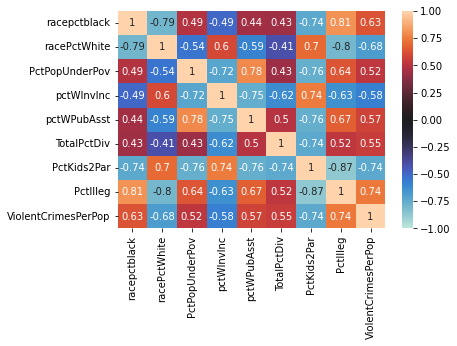
\includegraphics[width=10cm]{Heatmap.png}
\caption{The heat map for our attributes}
\label{fig:heatmap}
\end{figure}
\\
\\The first two attributes from the race category indicate that in cities in which there is a higher black population, there is a relatively strong positive correlation with the output attribute, violent crimes per 100K people. Similarly, we can say the same for cities with a higher white population (except it has a relatively strong negative correlation). There is no racism intended with these two statements, it is simply a reflection of the data.
\\
\\From the familial attributes, the first attribute PctKids2Par has a -0.74 correlation with violent crime, which translates to "the more kids that grow up with two parents in the household, the less violent crime there will be". PctIlleg is a very similar attribute that has the same correlation magnitude, but is negative instead of positive. Both of these attributes show how family incompleteness has a high correlation with violent crime.
\\
\\From the wealth attributes, the PctPopUnderPov and pctWPubAsst will be of high interest to politicians, as poverty and low income are traits generally associated with higher crime. These attributes have 0.52 and 0.57 correlation values with violent crime per 100K, which demonstrate an average magnitude of correlation. In other words, the correlation is not strong enough to be linear, but not weak enough to be irrelevant for use. Hence, we felt comfortable including these two attributes as inputs into our model. In addition, pctWInvInc could show the upper bound of the wealth of a community, which makes this attribute a good one to use when predicting violent crime.
\section{Algorithm Design}
\\The pair plot below is a visual display of the data set. The bottom row contains the input attributes on the x-axis and violent crimes per 100K on the y-axis. Through visual inspection, it can be determined that there is no strong linear or polynomial relationship between any of the variables and the output. However, because our inputs are all numeric values, we felt that a linear regression model would be a good model to employ. Knowing that we would be slightly underfitting our linear regression model, we needed to build a model that could deal with the data on a higher level with more accuracy. Hence, in addition to a linear regression model, we also decided to develop a neural network model.
\begin{figure}[H]
\centering
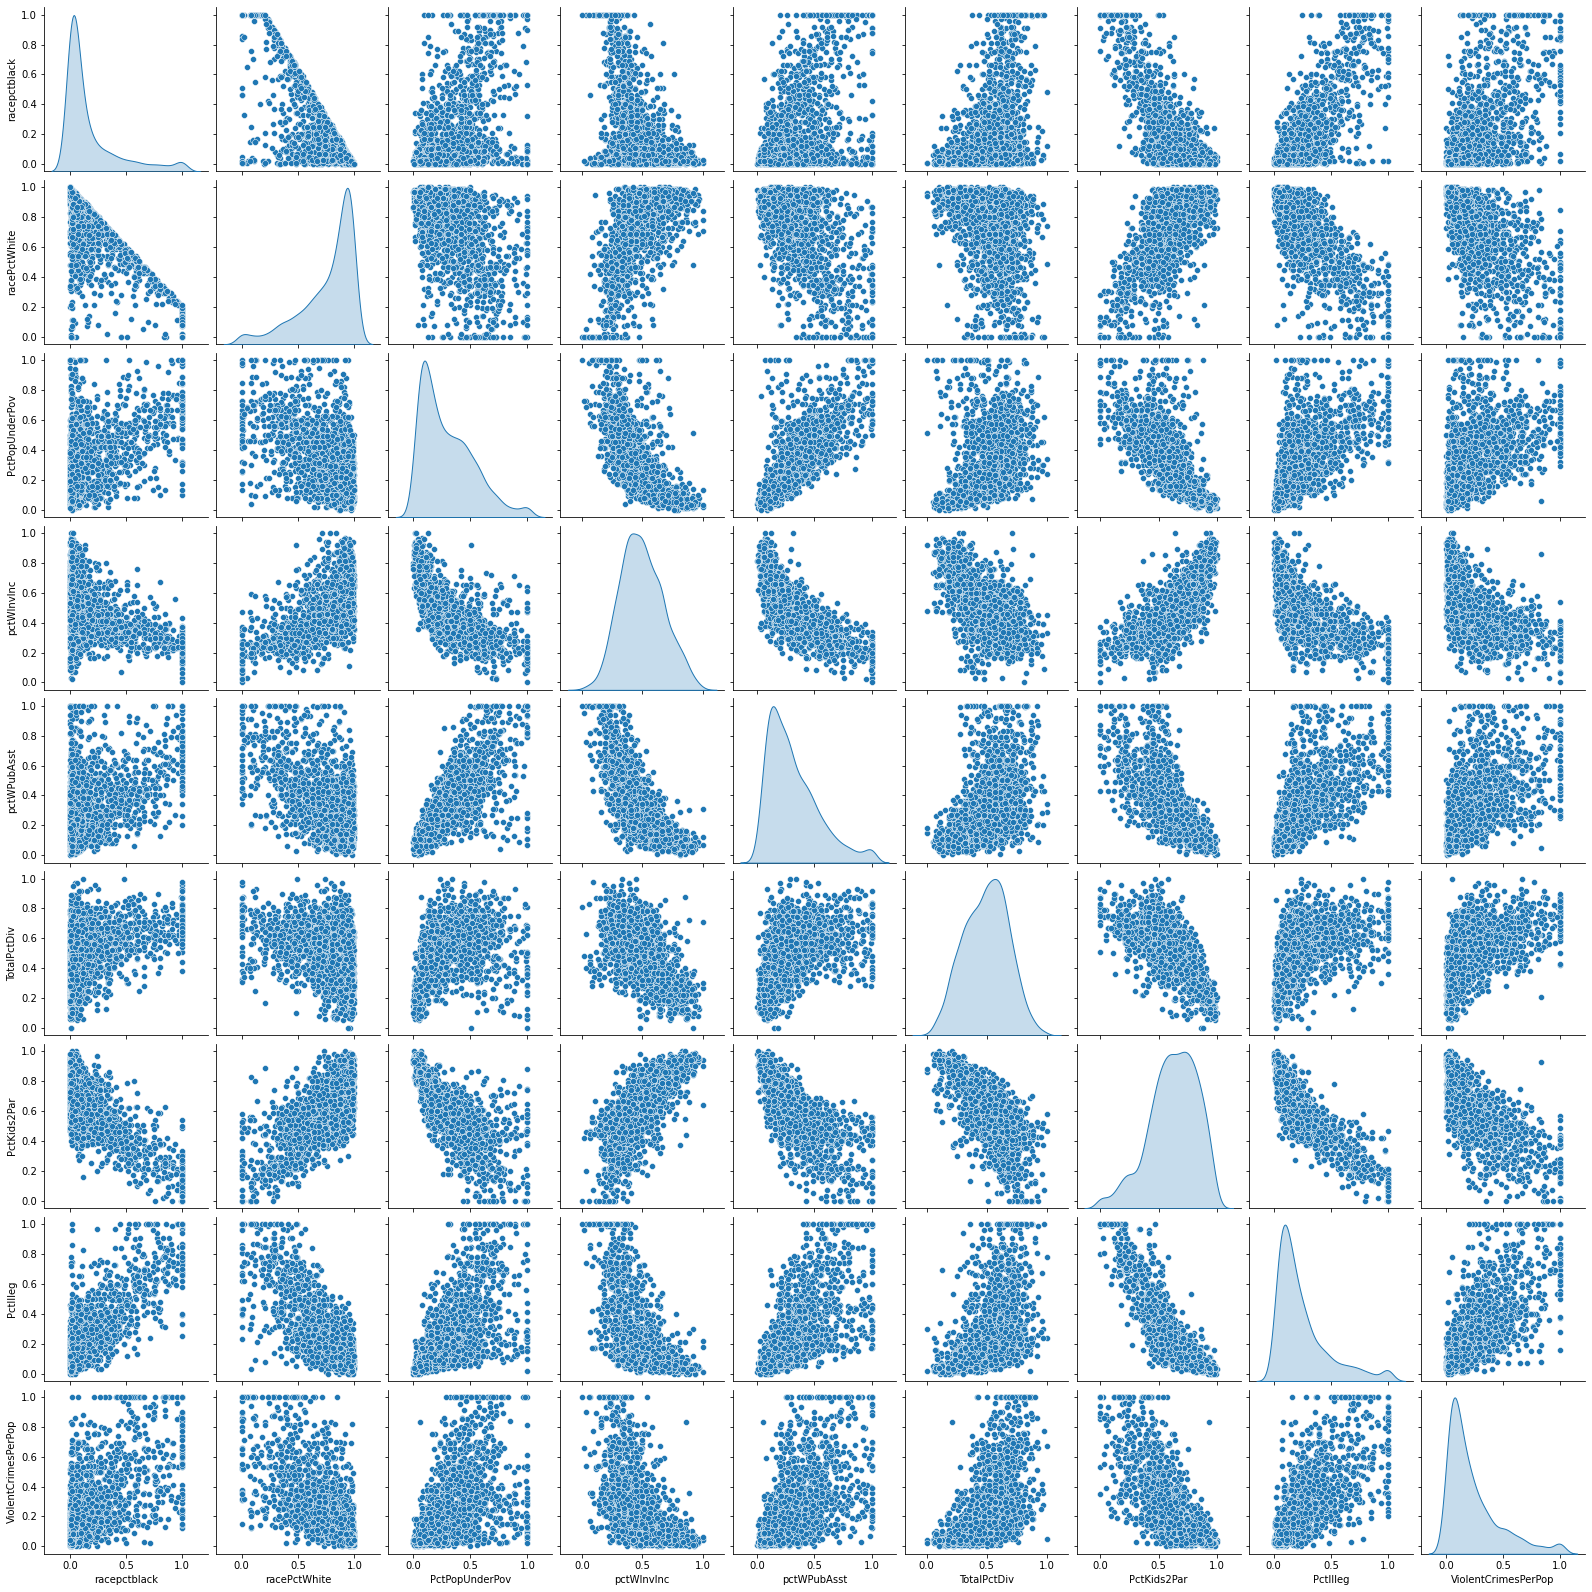
\includegraphics[width=0.4\textwidth]{Pairplot.png}
\caption{\label{fig:pairplot}The pair plot for our attributes}
\end{figure}

\subsection{Linear Regression Models}
\\We made four different linear regression models:
\\
\\ Familial Attributes vs. Violent Crimes Per 100K
\\ Wealth Attributes vs. Violent Crimes Per 100K
\\ Race Attributes vs. Violent Crimes Per 100K
\\ All Eight Attributes vs. Violent Crimes Per 100K
\\
\\We used the mean squared error metric to quantify the accuracy of our models. Specifically, we used k-fold Cross Validation with 10 splits of the data to generalize our linear regression model and obtain an average mean squared error. In other words, we implemented ten iterations, each using a different split of training and testing data, and calculated the mean squared error in each iteration, and then found the average of errors.

\subsection{Neural Network Models}
\\Like the linear regression models, we also made the same four neural network models. The main reason for this was to allow for better comparison of the two models when evaluating the results. 
\\
\\ Each of our four neural network models has five total layers: the input layer, three hidden layers, and the output layer. The number of nodes in the input layers is the number of input attributes and depends on the model we are using. The three hidden layers have 40, 10, and 4 nodes respectively. The output layer has one node, which contains our prediction. All layers expect the output layer use the ReLU activation function, and the learning rate is 0.01. Our output layer does not have an activation function because we want to provide a numeric prediction, rather than a probability (which is what an activation function provides).
\\
\\We also used the same metric to quantify the accuracy of the models: mean squared error. We used k-fold Cross Validation with 10 splits of the data, and using the same iterative implementation as in the linear regression model, calculated a value for the average mean squared error.

\section{Experiment Results}
\subsection{Comparison of Different Models}
\\The table below contains our numerical results. The left column specifies which model we are talking about. The middle column and right column provide the average mean squared error for the linear regression model and neural network model, respectively, for the model specified in the left column.
\begin{table}[H]
    \centering
    \begin{tabular}{ |p{3cm}||p{6cm}|p{5.5cm}|  }
     \hline
     \multicolumn{3}{|c|}{Model Comparisons} \\
     \hline
     Model Category & Linear Regression Average MSE & Neural Network Average MSE\\
     \hline
     Family & 0.0223 & 0.0214\\
     Wealth & 0.0337 & 0.0309\\
     Race & 0.0278 & 0.0273\\
     All & 0.0210 & 0.0179\\
     \hline
\end{tabular}
\caption{\label{tab:widgets}Average MSE for Every Linear Regression and Neural Network Model}
\end{table}
\\
\\For the family model, the linear regression average mean squared error (LRAMSE) was 0.0223, compared to the neural network average mean squared error (NNAMSE), 0.0214. This indicates that the neural network model is slightly more accurate when predicting violent crime given only the familial attributes.
\\
\\Similarly, the NNAMSE for the wealth model was slightly lower than the LRAMSE for the wealth model, with values of 0.0309 and 0.0337, respectively, indicating that the neural network model is more accurate when predicting violent crime rate given only wealth attributes.
\\
\\Comparing the average mean squared errors for the race attributes gives us different results than the prior two. The LRAMSE for the race model was 0.0278, which is minutely larger than the NNAMSE, 0.0273. The difference between these two mean squared errors, 0.0005, is negligible. This indicates that while the neural network technically was more accurate (by 0.0005), the predictions made by either model would be relatively the same.
\\
\\Looking at the individual models (predicting violent crime per 100K given only family, wealth, or race attributes), it can be seen that the model using the familial attributes would provide the most accurate results, as they have the smallest average mean squared error values for both the linear regression and neural network models. However, the model using the race attributes would provide the most consistent results across both models, as the difference in the average mean squared errors across both models is 0.0005, as stated above.
\\
\\Now, let us compare the average mean squared errors for the model that uses all eight input attributes to predict violent crime per 100K. The LRAMSE is 0.0210, which is significantly larger than the NNAMSE, 0.0179. This clearly indicates that when using all the attributes to predict violent crime, the neural network model outperforms the linear regression model.
\\
\\Overall, the data above establishes that the neural network model outperforms the linear regression model, in some cases significantly and in other cases minutely, for every model (family, wealth, race, and all). This is not surprising, as the relationships between our chosen input attributes and output variable were not completely linear. In general, using more attributes to predict violent crime per 100K yielded more accurate results. This may reflect that the eight attributes we selected are not completely independent. For instance, let's say that incomplete families are more common in certain races; a higher percentage of that race would lead to more incomplete families in the community, which consequently means more people relying on public assistance income. \href{https://www.census.gov/prod/1/statbrief/sb93_2.pdf} {This statistical brief} shows this very idea, displaying that the number of single family households in the African American community were increasing every decade until 1991, which is around the time the data in our data set was collected.
\\
\\Below, in Figures 3 and 4, you can see a visual plot representations of our algorithm's execution. The first image is obtained by executing the all attributes linear regression model. The second image is obtained by executing the all attributes neural network model. In both images, the red represents the actual values of our output variable, violent crimes per 100K, and the blue represents our predicted value for violent crimes per 100K. Executing the individual category LR and NN models (family, wealth, and race) will produce similar plots.
\begin{figure}[H]
\centering
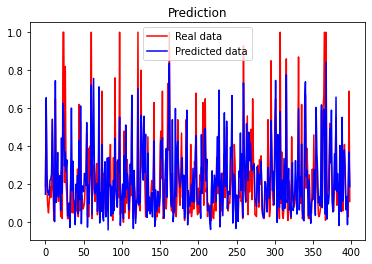
\includegraphics[width=8cm]{pred_all.png}
\caption{Predictions made by the linear regression all attributes model}
\label{fig:hotbo}
\end{figure}

\begin{figure}[H]
\centering
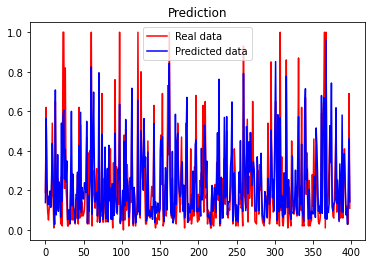
\includegraphics[width=8cm]{pred_nn.png}
\caption{Predictions made by the neural network all attributes model}
\label{fig:hotbo}
\end{figure}
\\
\\Through visual inspection, we can see that in general, the blue is overlapping the red, which indicates a good degree of accuracy in the predictions. In cases where the actual crime rate normalized value was above 0.8, the predictions were lower and couldn't reach up to the point of 0.8. Taking a look at the region of the plots where the actual normalized crime rate was a little under 0.1, we can see that the linear regression model made predictions lower than the actual values and the neural network model made predictions higher than the actual values.
\\
\section{Conclusion and Discussion}
\subsection{Limitations and Future Actions}
\\One of the limitations of our machine learning algorithms is that the prediction for violent crimes per 100K that our algorithm makes is not an actual numeric value, such as 100. It is a normalized value, in the form of a decimal between 0 and 1. The reason for this is that the data set we used contained values that were already normalized using an unsupervised equal-interval binning method, rather than including the original numeric values. Hence, the predictions are also normalized. A normalized prediction value will not be very useful to politicians, for example, when evaluating crime rates in communities, as it is unable to be interpreted. However, we recently discovered the unnormalized data set that contains numeric values instead of normalized values. In the future, we can take this unnormalized data set, apply the aforementioned unsupervised equal-interval binning method to normalize the data set, then call our machine learning algorithm to predict a normalized value, and finally use an inverse transformation technique to convert this normalized prediction value into a numeric predicted value. This will allow politicians, or whoever is using our algorithm, to better interpret the results na
\\
\\Another course of action we can take in the future is to implement polynomial regression models in addition to linear regression and neural network models. The resulting average mean squared values and visual prediction plots will allow us to identify where a polynomial regression ranks accuracy wise in comparison to the linear regression and neural network models we have already implemented.

\subsection{Discussion}
\\From our research, we discovered that crime rates vary across communities throughout the United States. This is because different factors impact the crime rate in different communities. It is important to do whatever we can to reduce violent crime, but the problem is that there isn't one single solution that can accomplish this, meaning that changes enacted at the federal level, or even the state level, will not be of much use. The best course of action is to tackle the issue at the local level on a community by community basis. This is where our algorithm comes in. Local lawmakers can use our algorithm to predict future violent crime rates given differing levels of the input attributes to identify what specific factors lead to higher violent crime in their communities. After identifying what specific factors impact the violent crime rate in their community, local governments can then take appropriate actions to address those factors and reduce violent crime.
\\
\\One form of the aforementioned appropriate actions is for local governments to divert resources to community organizations. Through research, we discovered that community organizations and communal involvement do in fact reduce violent crime. For example, creating an organization to help people in a community find jobs will eventually result in those individuals obtaining a source of income and not having to resort to violent crimes such as armed robbery to obtain money. While more research is needed to improve our public response to crime, supporting and reforming the community to help drive the reduction in crime is an excellent place to start.

\clearpage
\bibliographystyle{alpha}
\bibliography{sample}

\end{document}
